\section{【实现】内核态切换到用户态}\label{ux5b9eux73b0ux5185ux6838ux6001ux5207ux6362ux5230ux7528ux6237ux6001}

在kern/init.c中的switch\_test函数完成了内核态\textless{}--\textgreater{}用户态之间的切换。内核态切换到用户态是通过swtich\_to\_user函数,执行指令``int
T\_SWITCH\_TOU''。当CPU执行这个指令时,由于是在switch\_to\_user执行在内核态,所以不存在特权级切换问题,硬件只会在内核栈中压入Error
Code(可选)、EIP、CS和EFLAGS(如下图所示),然后跳转到到IDT中记录的中断号T\_SWITCH\_TOU所对应的中断服务例程入口地址处继续执行。通过2.3.7小节``中断处理过程''可知,会执行到trap\_disptach函数(位于trap.c):

\begin{lstlisting}
case T_SWITCH_TOU:
if (tf->tf_cs != USER_CS) {
//当前在内核态,需要建立切换到用户态所需的trapframe结构的数据switchk2u
switchk2u = *tf;
switchk2u.tf_cs = USER_CS;
switchk2u.tf_ds = switchk2u.tf_es = switchk2u.tf_ss = USER_DS;
switchk2u.tf_esp = (uint32_t)tf + sizeof(struct trapframe) - 8;
   //设置EFLAG的I/O特权位,使得在用户态可使用in/out指令
switchk2u.tf_eflags |= (3 << 12);
    //设置临时栈,指向switchk2u,这样iret返回时,CPU会从switchk2u恢复数据,
//而不是从现有栈恢复数据。
    *((uint32_t *)tf - 1) = (uint32_t)&switchk2u;
}
\end{lstlisting}

这样在trap将会返回,在\_\_trapret:中,根据switchk2u的内容完成对返回前的寄存器和栈的回复准备工作,最后通过iret指令,CPU返回``int
T\_SWITCH\_TOU''的后一条指令处,以用户态模式继续执行。

\begin{figure}[htbp]
\centering
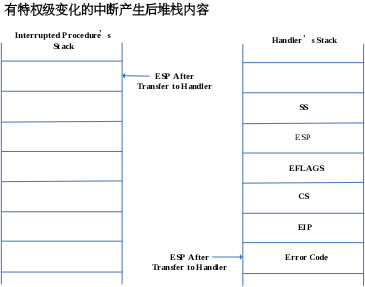
\includegraphics{figures/3.5.5.1.png}
\caption{3.5.5.1}
\end{figure}
